\documentclass[10pt]{article}
\usepackage[margin=0.65in]{geometry}
\usepackage{graphicx}
\usepackage{amsmath}
\usepackage{booktabs}
\usepackage{hyperref}
\title{Compiled-expression bridge for the genus-2 doubling intermediates}
\author{Source-bound finite review packet}
\date{25 October 2026}
\begin{document}\maketitle\small
The script \texttt{run.py} verifies the complete pinned Rust source hash, extracts
the exact \texttt{N1,N2,B,N5,N6,A,C} expression statements from
\texttt{double22\_weighted\_variant}, and checks that production
\texttt{double22\_weighted} passes the squared-$w$ flag. It compiles those
statements with a minimal $\mathbf F_5$ field implementation, then independently
evaluates the pinned author Magma expressions on every tuple
$(q,r,s,t,z,w,a_2,a_3)\in\mathbf F_5^8$.

\begin{center}\begin{tabular}{lr}\toprule
Quantity & Count\\\midrule
All tuples & 390,625\\
$B\ne0$ tuples & 312,500\\
Pinned $W^2$ expression mismatches & 0\\
Synthetic $W^1$ mutation: $N6$ mismatches & 187,500\\
Synthetic $W^1$ mutation: $A$ mismatches & 120,000\\
Synthetic $W^1$ mutation: $C$ mismatches & 150,000\\\bottomrule
\end{tabular}\end{center}
\begin{center}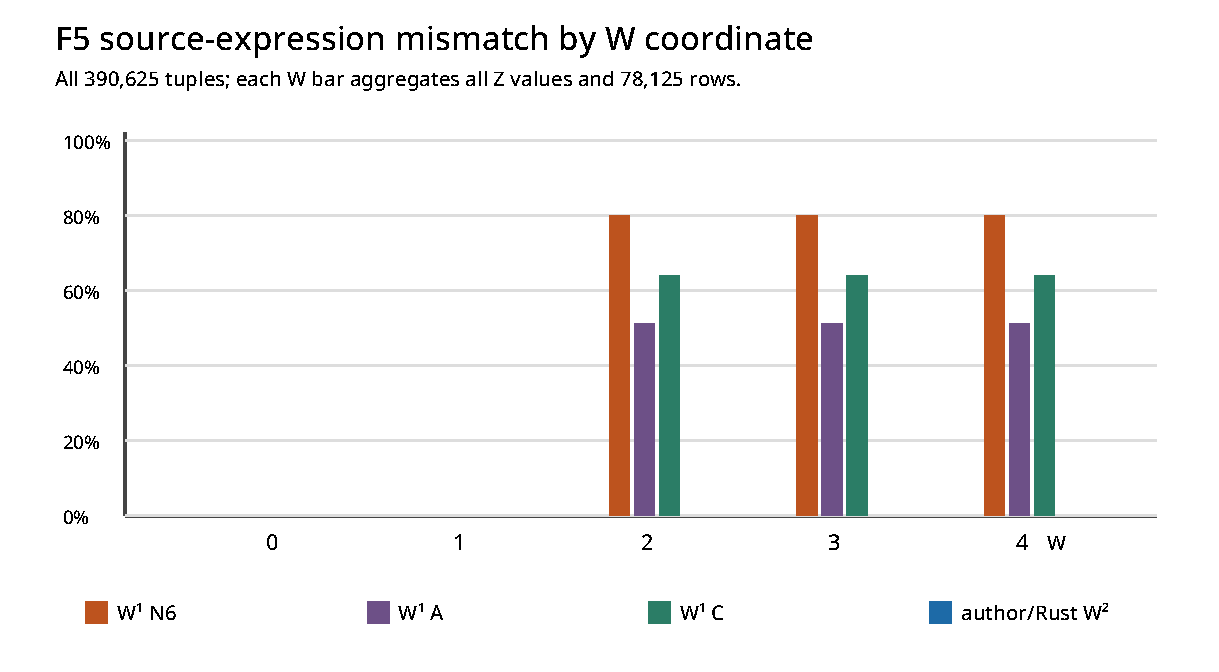
\includegraphics[width=0.76\textwidth]{GRAPH.pdf}\end{center}
The graph and \texttt{ROWS.csv} retain each $(z,w)$ stratum, including
$B=0$ and zero-coordinate diagnostics. The production function returns before
computing $N5,N6,A,C$ when $B=0$; those rows check only the extracted algebraic
continuation. The check spans unconstrained tuples, not an assertion that every
tuple represents a valid divisor on a smooth curve.

This finite result binds an exact source excerpt and its compiled arithmetic
to the author expressions. It does not establish equivalence of the full
production binary, exceptional-case dispatch, output divisor, or $\operatorname{Pic}^0$
group law. The separate Lean packet proves polynomial coefficient identities,
but a universal formal Rust-semantics bridge remains open. No cost row changes.

Source digests, full replay criteria, and row-stream hashes are in
\texttt{RESULT.json}; see \texttt{ROWS.csv} and \texttt{run.py} for replay.
\end{document}
